\section{Reverse Problem Discussion}

\subsection{Hodograph approaches and historical remarks}

\subsubsection{Newton, uniqueness, and asserted conics}

From the \emph{Principia} viewpoint (1687), Newton gives a geometric proposition-chain establishing both directions: conic with force at a focus $\Rightarrow$ inverse-square law, and inverse-square centripetal attraction $\Rightarrow$ conic orbits (ellipse/parabola/hyperbola by regime) \cite{newton1687principia,chandrasekhar1995principia}. What he does \emph{not} provide is a modern initial-value existence/uniqueness theorem for the inverse problem; the argument is synthetic and limit-geometric (ultimate ratios), not an ODE well-posedness proof.

In parallel, early Continental analysts (late 17th to early 18th century) reduced the central-force problem by $u(\theta)=1/r$, yielding Binet's equation. For $F(r)=-\mu/r^2$:
\begin{equation}
  u''(\theta)+u=\frac{\mu}{h^2},
\end{equation}
with solution
\begin{equation}
  u(\theta)=\frac{\mu}{h^2}\Bigl(1+e\cos(\theta-\theta_0)\Bigr),
\end{equation}
i.e. a conic in polar form. However, deriving this form by itself is not a substitute for a uniqueness theorem: without an existence/uniqueness framework, one has not yet formalized exclusion of other possible local branches/continuations. Historical accounts of this transition to differential methods are discussed by Nauenberg (2003) \cite{nauenberg2003keplerarea}.

So the modern statement ``initial data determine a unique orbit'' is best read as a reconstruction of Newton's practice rather than a theorem he states in contemporary form. The same caution applies to early Continental differential reductions: the orbit equation gives candidate solution families, while later uniqueness theory is what formally secures single-orbit determinacy from initial data. Likewise, hodograph language is absent in the \emph{Principia} (1687) and appears later with Hamilton (1847). Rigorous local existence/uniqueness theorems for ODEs were developed much later (Cauchy in the 1820s; then Lipschitz/Picard--Lindel\"of in the late 19th century, roughly the 1870s--1890s), i.e. more than a century after 1687.

\subsubsection{Hamilton's circular hodograph for the inverse-square law}

Hamilton introduced the hodograph in 1847 as the curve traced by the tip of the velocity vector $\mathbf v(t)$ in velocity space, and showed that for motion under a central inverse-square force the hodograph is a circle \cite{hamilton1847hodograph}.

Write the dynamics as
\[
  \ddot{\mathbf r}=-\frac{\mu}{r^2}\,\hat{\mathbf r},
  \qquad
  h:=r^2\dot\theta=\text{const}.
\]
Reparametrize by $\theta$:
\begin{equation}
  \frac{d\mathbf v}{d\theta}
  =
  \frac{d\mathbf v}{dt}\frac{dt}{d\theta}
  =
  \ddot{\mathbf r}\,\frac{r^2}{h}
  =
  -\frac{\mu}{h}\,\hat{\mathbf r}.
\label{eq:hodo-step1}
\end{equation}
Using the polar-frame identity
\[
  \frac{d\hat{\boldsymbol\theta}}{d\theta}=-\hat{\mathbf r},
\]
equation~\eqref{eq:hodo-step1} becomes
\begin{equation}
  \frac{d\mathbf v}{d\theta}
  =
  \frac{\mu}{h}\frac{d\hat{\boldsymbol\theta}}{d\theta}.
\label{eq:hodo-step2}
\end{equation}
Integrating once gives
\begin{equation}
  \frac{d}{d\theta}\!\left(\mathbf v-\frac{\mu}{h}\hat{\boldsymbol\theta}\right)=0
  \quad\Longrightarrow\quad
  \mathbf v=\mathbf C+\frac{\mu}{h}\hat{\boldsymbol\theta}.
\label{eq:hodo-step3}
\end{equation}
with constant vector $\mathbf C$.
Because $\|\hat{\boldsymbol\theta}\|=1$,
\[
  \|\mathbf v-\mathbf C\|=\frac{\mu}{h}.
\]
Hence the hodograph (the tip of $\mathbf v$ in velocity space) is a circle of radius $\mu/h$, centered at $\mathbf C$.
Later expositions (notably Maxwell, 1877) emphasize that the hodograph circle is not only a consequence of inverse-square attraction, but also a practical route toward reconstructing the orbit and diagnosing the force law when combined with angular momentum conservation \cite{maxwell1877mattermotion,derbes2001reinventing}. In this pedagogical tradition (Hamilton, 1847 $\to$ Maxwell, 1877 $\to$ Feynman, 1964, with later refinements), one studies both Kepler problems: direct (force $\Rightarrow$ orbit) and inverse (orbit laws $\Rightarrow$ force) \cite{derbes2001reinventing}.

\subsubsection{Feynman's Lost Lecture, strengths, and later repairs}

Feynman's 1964 lecture re-popularized the hodograph method for teaching: first establishing a circular hodograph for inverse-square attraction, then reconstructing the conic orbit geometrically \cite{goodstein1996feynman}. Later work, including Derbes (2001), clarified missing details in tangent placement and invariants; in particular, angular momentum conservation is the extra ingredient that fixes line placement and scale \cite{derbes2001reinventing}. More recent refinements, including van Haandel--Heckman (2009) and follow-up work by Cari\~nena--Ra\~nada--Santander (2016), may be read as using either (i) the directrix circle centered at the second focus, or (ii) an equivalent directrix-circle/hodograph picture centered at the force center, with a $\pm 90^\circ$ rotation between velocity and geometric proxy \cite{vanhaandelheckman2009teaching,carinena2016newlook}. CNRNS16 emphasizes that the force-center version gives a cleaner Feynman-style transformation.

In our constructions (\Cref{fig:hyperbola,fig:parabola-proof2}), the auxiliary circle has the same dual role. In particular, from the local identity used in \Cref{lem:product-identity},
\[
  FH\cdot FK' = b^2,
  \qquad
  F'\!A' = FK',
\]
so $\overrightarrow{F'\!A'}$ and $\overrightarrow{FK'}$ are colinear with opposite orientation and equal magnitude. Hence one can use the auxiliary-circle data with either center choice ($F$ or $F'$) as a hodograph proxy, corresponding to a $+90^\circ$ or $-90^\circ$ rotation. For the parabola, the same logic yields four equivalent rotated-hodograph constructions; Derbes' choice is one of them (his $C_4$ circle). The remaining step is the energy classification: $E<0$ gives an ellipse, $E=0$ the parabolic limit, and $E>0$ a hyperbola.

\subsection{Our approach (Newton-style discretization built on the hodograph circle)}

We take as given (from Section~8.1) the hodograph-circle fact: for planar motion under a central inverse-square force, the hodograph of $\mathbf v(t)$ is a circle in velocity space.

Our goal is to recover the orbit form $r(\theta)$ by a finite-step argument aligned with Newton's impulse-triangle logic, minimizing reliance on continuous calculus.

\subsubsection{Hodograph-radius analysis and translated-circle reconstruction}

Assume planar motion under a centripetal acceleration toward $F$:
\begin{equation}
  a=\frac{k}{r^2},
  \qquad
  r=FA,
\end{equation}
and constant specific angular momentum
\begin{equation}
  L=r^2\dot\theta.
\end{equation}
Fix a small time step $\Delta t$, with consecutive points $B\to A$ on the orbit, $BR\perp FA$, and the translated $\Delta t$-scaled hodograph geometry in which
\begin{equation}
  OM=BR+OR'.
\end{equation}
Define
\begin{equation}
  u:=\frac{k}{L}.
\end{equation}

\begin{figure}[t]
  \centering
  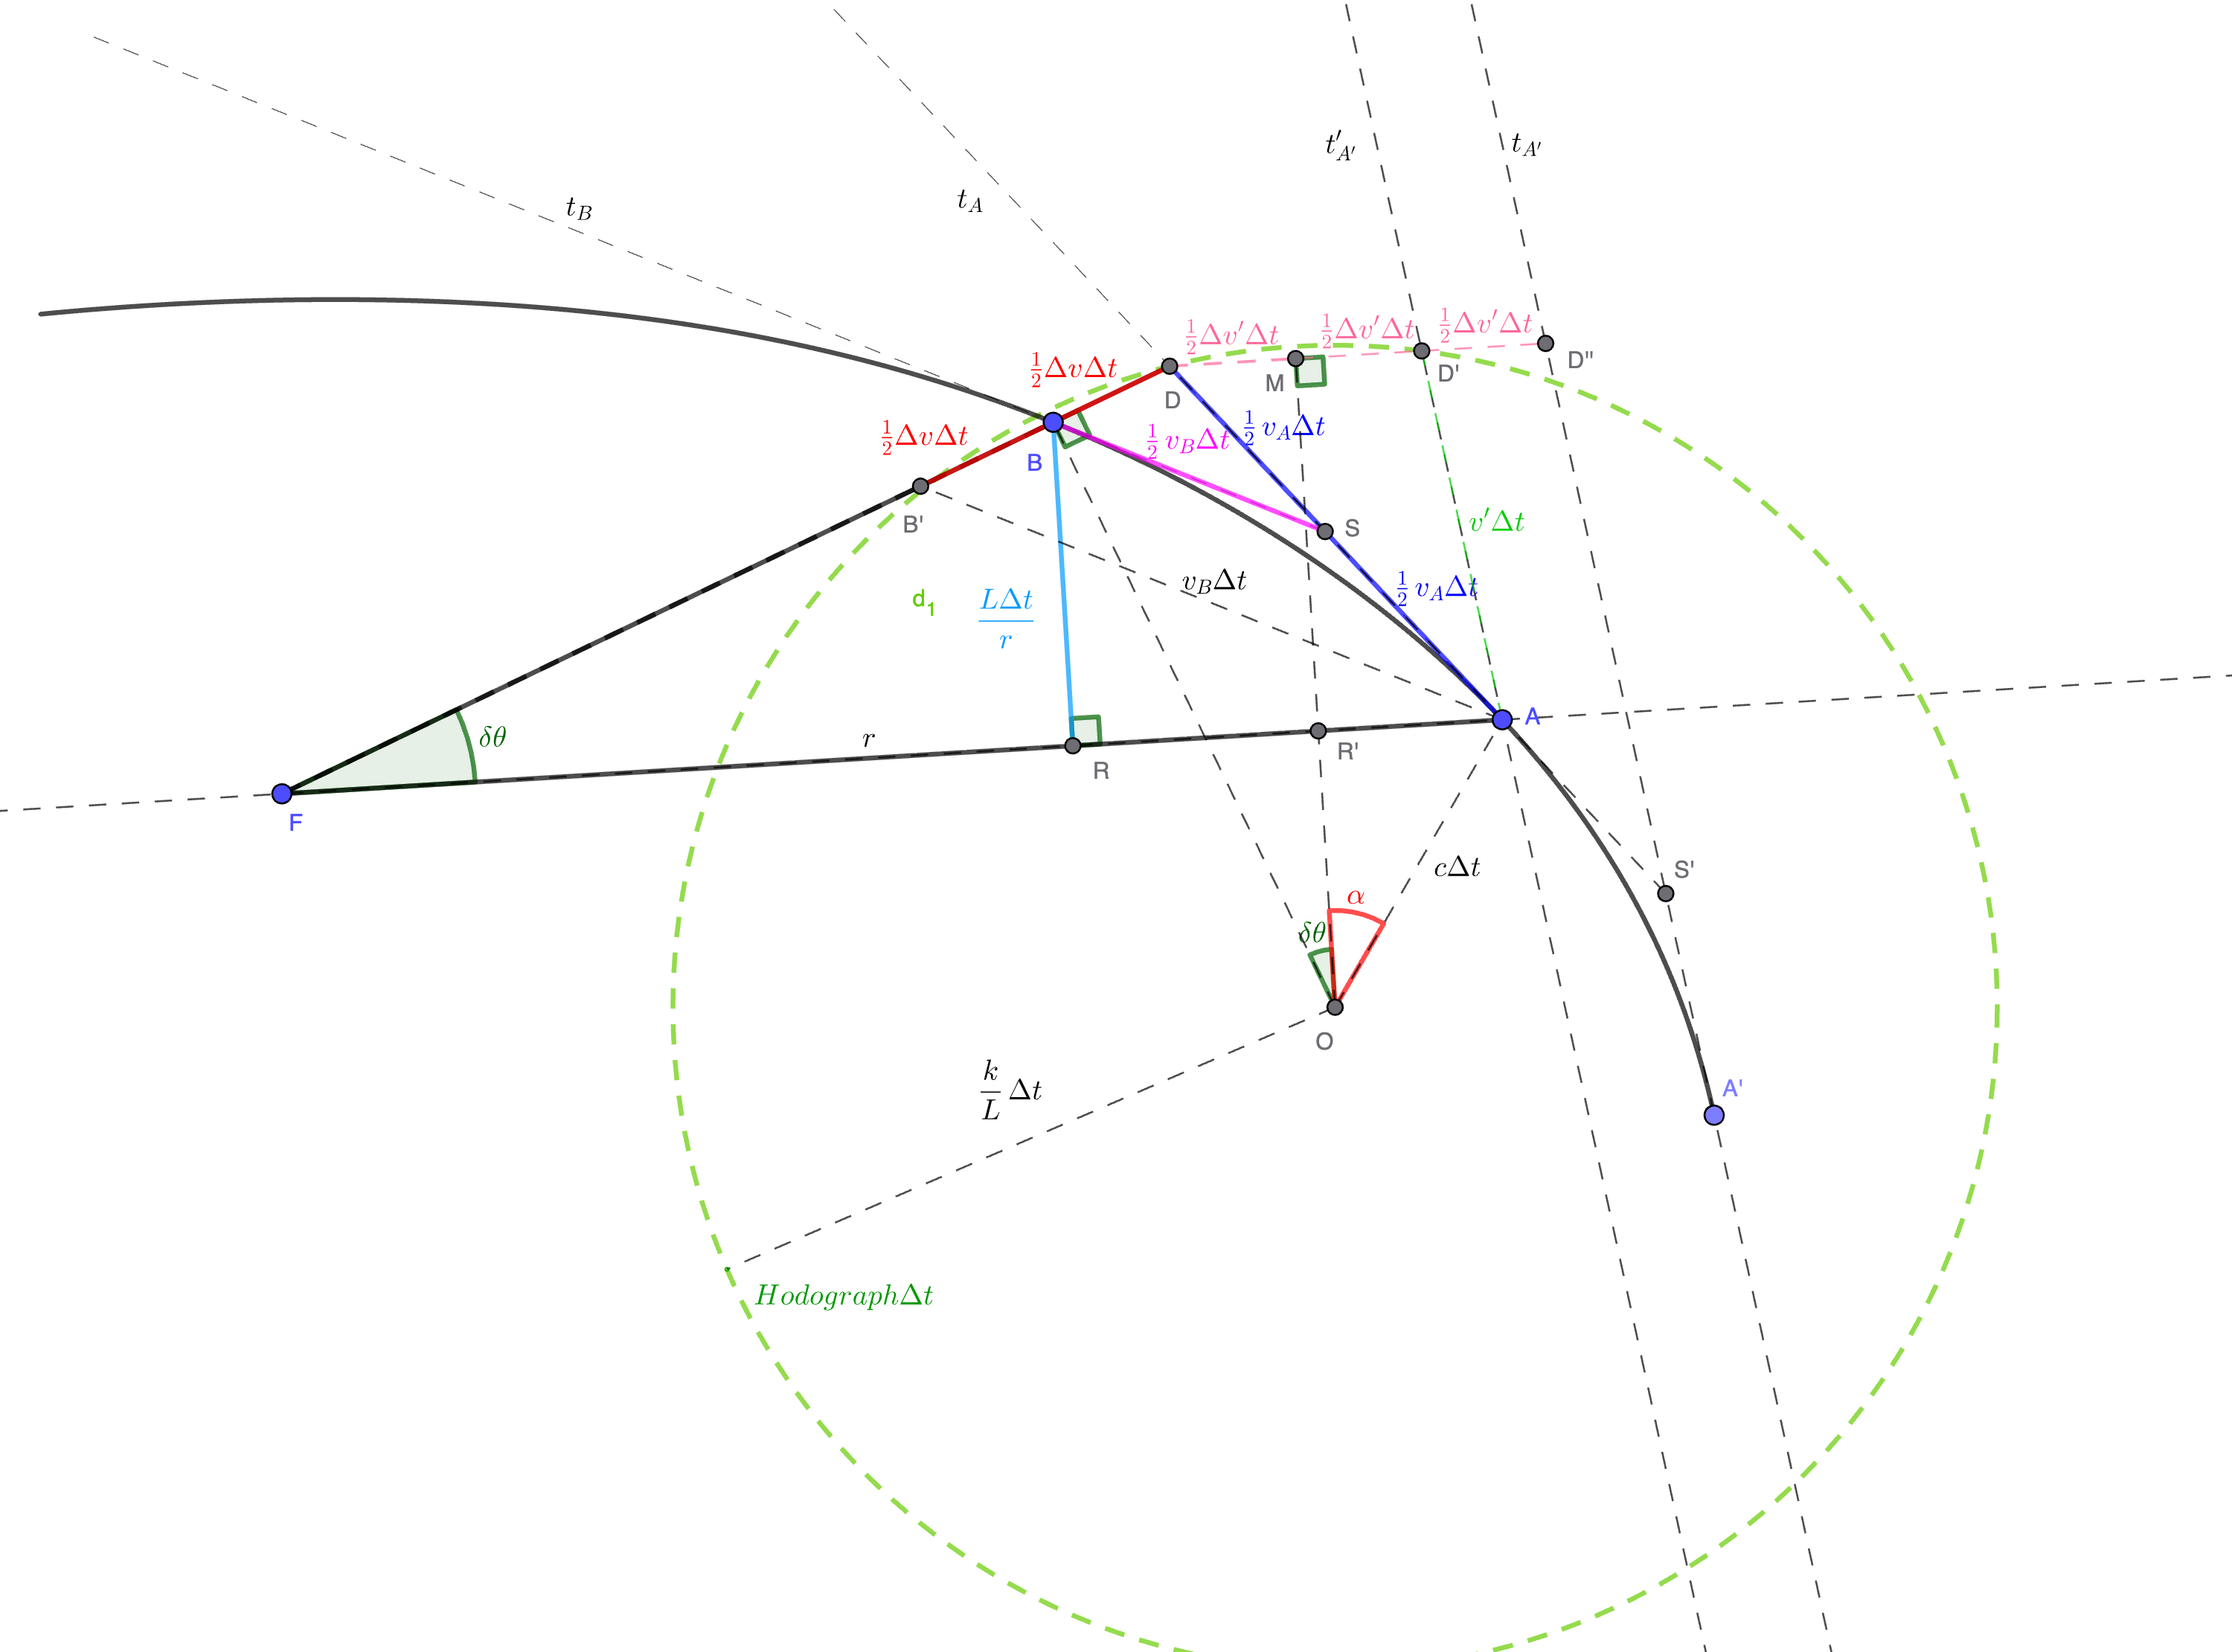
\includegraphics[width=0.95\linewidth]{assets/images/inverse_problem.png}
  \caption{Inverse-problem construction in Section~8.2.1: previous/current/next velocities ($V_{A'},V_A,V_B$), each scaled by $\Delta t$, are shown on the translated $\Delta t$-scaled hodograph circle, with decomposition $OM=BR+OR'$.}
  \label{fig:inverse-problem}
\end{figure}

\begin{proposition}[Hodograph-radius analysis $\Rightarrow$ conic form]
\label{prop:inverse-hodograph-proof}
With the notation of \Cref{fig:inverse-problem}:
\begin{enumerate}[label=(\roman*),leftmargin=*]
  \item the hodograph of $\mathbf v$ is a circle of radius $u$ (hence the $\Delta t$-scaled hodograph circle has radius $u\Delta t$);
  \item if the fixed shift satisfies $OR'=c\,\Delta t\cos\alpha$, then
  \begin{equation}
    \frac1r=\frac{k}{L^2}-\frac{c}{L}\cos\alpha
    \quad\Longleftrightarrow\quad
    r(\alpha)=\frac{p}{1-\varepsilon\cos\alpha},
    \qquad
    p=\frac{L^2}{k},
    \quad
    \varepsilon=\frac{cL}{k}=\frac{c}{u}.
  \end{equation}
  \item
  \begin{equation}
    \begin{aligned}
      \frac{c}{u}<1,\;=1,\;>1
      &\Longleftrightarrow
      \text{velocity-origin inside/on/outside hodograph circle}\\
      &\Longleftrightarrow
      \text{ellipse/parabola/hyperbola}.
    \end{aligned}
  \end{equation}
\end{enumerate}
\end{proposition}

\begin{proof}
In \Cref{fig:inverse-problem}, the previous, current, and next velocities ($V_{A'},V_A,V_B$) are placed together in velocity space after scaling by $\Delta t$; this is exactly the translated $\Delta t$-scaled hodograph circle used in the relations below.

\textbf{1) $\Delta v$ depends only on $\Delta\theta$.}
Over a short interval $\Delta t$,
\[
  \Delta v=a\,\Delta t=\frac{k}{r^2}\Delta t.
\]
From $L=r^2\dot\theta$, one has $\Delta t=\frac{r^2}{L}\Delta\theta$. Hence
\begin{equation}
  \Delta v=\frac{k}{r^2}\cdot\frac{r^2}{L}\Delta\theta=\frac{k}{L}\Delta\theta=u\,\Delta\theta,
  \qquad
  \frac{\Delta v}{\Delta\theta}=u\ \text{(constant)}.
\label{eq:inverse-step1}
\end{equation}

\textbf{2) Hodograph-circle conclusion.}
Because the force is central, $\Delta\mathbf v$ is radial inward. As $FA$ turns by $\Delta\theta$, the direction of $\Delta\mathbf v$ turns by the same $\Delta\theta$, while its magnitude is $u\,\Delta\theta$ by \eqref{eq:inverse-step1}. Thus the velocity-tip polygon is the equal-angle, equal-arc-length limit of an inscribed circle polygon, so the hodograph is a circle of radius $u$. Multiplying by $\Delta t$ gives
\begin{equation}
  OM=u\,\Delta t.
\label{eq:inverse-step2}
\end{equation}

\textbf{3) Tangential displacement.}
The tangential speed is $v_\theta=L/r$, hence
\begin{equation}
  BR=v_\theta\Delta t=\frac{L}{r}\Delta t.
\label{eq:inverse-step3}
\end{equation}

\textbf{4) Key geometry in the plot.}
From the translated-circle construction, $OM=MR'+OR'$ and $MR'=BR$, so
\begin{equation}
  OM=BR+OR'.
\label{eq:inverse-step4}
\end{equation}
Assume
\begin{equation}
  OR'=c\,\Delta t\cos\alpha.
\label{eq:inverse-step5}
\end{equation}
Substitute \eqref{eq:inverse-step2}, \eqref{eq:inverse-step3}, \eqref{eq:inverse-step5} into \eqref{eq:inverse-step4}:
\[
  u\Delta t=\frac{L}{r}\Delta t+c\Delta t\cos\alpha.
\]
Cancel $\Delta t$:
\[
  u=\frac{L}{r}+c\cos\alpha
  \quad\Longrightarrow\quad
  \frac1r=\frac{u}{L}-\frac{c}{L}\cos\alpha
  =\frac{k}{L^2}-\frac{c}{L}\cos\alpha.
\]
This is equivalent to
\[
  r(\alpha)=\frac{p}{1-\varepsilon\cos\alpha},
  \qquad
  p=\frac{L^2}{k},
  \quad
  \varepsilon=\frac{cL}{k}=\frac{c}{u}.
\]

\textbf{5) Classification by origin position in velocity space.}
The hodograph circle has radius $u$, and the velocity-origin offset has magnitude $c$. Hence the origin is inside/on/outside the hodograph circle according as $c<u$, $c=u$, $c>u$, i.e. $c/u<1,=1,>1$. Since $\varepsilon=c/u$, these are precisely $\varepsilon<1,=1,>1$, giving ellipse/parabola/hyperbola.
\end{proof}
